\documentclass[11pt,letterpaper]{article}

%%%%%%%%%%%%%%%%%%%%%%%%%%%%%%%%%%%%%%%%%%%%%%%%%%%%%%%%%%%%%%%%%%%%%%%%%
\pagestyle{plain}                                                      %%
%%%%%%%%%% EXACT 1in MARGINS %%%%%%%                                   %%
\setlength{\textwidth}{6.5in}     %%                                   %%
\setlength{\oddsidemargin}{0in}   %% (It is recommended that you       %%
\setlength{\evensidemargin}{0in}  %%  not change these parameters,     %%
\setlength{\textheight}{8.5in}    %%  at the risk of having your       %%
\setlength{\topmargin}{0in}       %%  proposal dismissed on the basis  %%
\setlength{\headheight}{0in}      %%  of incorrect formatting!!!)      %%
\setlength{\headsep}{0in}         %%                                   %%
\setlength{\footskip}{.5in}       %%                                   %%
%%%%%%%%%%%%%%%%%%%%%%%%%%%%%%%%%%%%                                   %%
%\newcommand{\required}[1]{\section*{\hfil #1\hfil}}                   %%
\renewcommand{\refname}{\hfil References Cited\hfil}                   %%
%\bibliographystyle{plain}                                             %%
%%%%%%%%%%%%%%%%%%%%%%%%%%%%%%%%%%%%%%%%%%%%%%%%%%%%%%%%%%%%%%%%%%%%%%%%%

%PUT YOUR MACROS HERE

\usepackage{amsmath}
\usepackage{amsfonts}
\usepackage{amssymb}
\usepackage{graphicx}
\usepackage{ulem}
\usepackage[hidelinks]{hyperref}


\title{Magnetometry}


\author{Ian Hunt-Isaak\\ \begin{small}
Partner: Corina Miner
\end{small}}

\begin{document}


\date{}
\maketitle
\section{} %1
\subsection{Ferromagnet}
Distinctive feature is a nonlinear M vs H curve that is not reversible. That is the curve displays hysteresis.
\subsubsection{Soft}
Soft magnets have a small remenant magnetization.
\subsubsection{Hard}
Hard ferroamgnets have a large remanant magnetization.
\subsection{Paramagnet}
A linear M vs H curve, with 0 remanent magnetization and reversible magnetization. Attracted to magnetic fields
\subsection{Diamagnet}
Repelled from magnetic fields. Linear M vs H that is reversible. Has a negative slope.
\section{} %2
In order to identify the samples we calculated their saturation magnetization per gram and compared that to values taken from the CRC handbook.
\subsection{Sample A}
Sample A was very soft and the curvature of the loop was lost as this curvature would be smaller than the resolution of the instrument. However at the highest applied field magnetization had flatlined so the average value of the magnetization at the extremes of the applied field were averaged to determine the saturation magnetization. From this we found the saturation magnetization per gram to $228.7\pm .6$ emu/g for sample A. The ferromagnetic material with the closest saturation magnetization per gram is Iron with a value of  $218.0$ emu/g.

\subsection{Sample C}
The data for sample C was fit to a Langevin function:
\begin{equation}
M(H)=N m\left(cos(\frac{m H}{k_b T})-\frac{k_b T}{m H}\right) = a\left(cos(b H)-\frac{1}{b H}\right)
\end{equation}
Fitting to this function we then determined the saturation magnetization as $M_s=\lim_{H\to\infty} M(H)$. By this method we found the magnetization per gram to be $57.7\pm 2$ emu/g. The literature value to which this is closest to is that of Nickel with has a value of $54.39$ emu/g. From this we identify sample C as Nickel.
\subsection{Uncertainty Budget}
\begin{table}[!h]
	\begin{center} 
		\begin{tabular}{|c|c|c|c|} \hline 
			Source & Type&  Error in Quantity  & Propagated Error  \\ \hline \hline
			Massing Sample & Random & .1 mg & Small \\ \hline
			Saddling & Random & M $\pm$ 5\%& N/A\\ \hline
			Calibration &  Systematic& N/A & N/A \\ \hline
            
			\hline
		\end{tabular}
        \caption{Uncertainty Budget for this work.}
	\end{center}
\end{table}
There error in the saddling becomes irrelevant as it affects both ends of the hystersis loop symmetrically and so shold cancel out the effects of eachother.
The dominant error ended up being the error in the fit coefficients which was enhanced by the division of the very small mass.
\section{} %3
The additional sample we investigated was Sample B. The method of investigation was exactly the same as for sample C. The issue however was that with sample B we were unable to reach saturation of the magnetization and so are less trusting of our value. In particular note that the residuals are more dramatic for Sample B than for C. 
By this method we found the magnetization per gram to be $192.9\pm 2$ emu/g. The literature value to which this is closest to is that of Cobalt with has a value of $168$ emu/g. From this we identify sample B as Nickel.
\subsection{Uncertainty Budget}

This sample was not one of the common objects and so we can't comment on how this relates to it's use.
\section{} %4
A vibrating sample magnetometer (VSM) works on Faraday's principle of Induction. The sample is surrounded by coils and rapidly vibrated under the applied magnetic field. Due to the field the sample will be magnetized and the movement of the sample will induce a voltage in the surrounding pickup coils. Using this induced voltage the coils can be used as a gradiometer to determine the magnetization of the sample.

While the VSM relies on macro-scale induction a SQUID magnetometer relies on quantum mechanical aspects of induction to measure magnetization with a resolution as fine as $10^{-15}$ T. As can be seen in Fig. \ref{fig:SQUID} a SQUID magnetometer consists of a superconducting ring with one or two non superconducting josephson junctions. The consequence of this setup is that the flux through the ring is quantized in amounts of the flux quantum $\Phi_0 \cong 2.06 \cdot 10^{-15}$Tm$^2$. Using specialized electronics the number of flux quanta passing through the loop can be determined and from this the magnetization of the sample worked out. SQUID magnetometry is in the same spirit as VSM but taken to an extreme and utilizing the quantization effects of quantum mechanics.
\begin{figure}[h!]
  \centering
      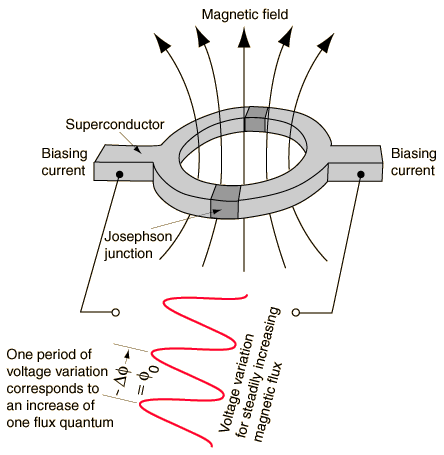
\includegraphics[scale=.8]{SQUID.png}
      \caption{Image from {\url http://hydrogen.physik.uni\-uppertal.de/hyperphysics/hyperphysics/hbase/solids/imgsol/squide.gif}}
      \label{fig:SQUID}
\end{figure}
\section{}%5
A Hall Effect Gaussmeter works on the principle of the Lorentz force of a magnetic field acting on a moving charge. Placing a metallic strip of significant width in a magnetic field and running current through it will cause the Lorentz force to act on the charge carriers in the metal. The component of the field normal to the surface of the strip will cause a charge imbalance to develop accross the width of the strip, this can be visualized in Fig. \ref{fig:hall_effect}. By measuring the voltage generated by the charge imbalance, $V_H$ in Fig. \ref{fig:hall_effect}, and knowing the magnitude of the current and properties such as the charge carrier density of the material we can determine the magnitude of the magnetic field normal to the strip. The fact that a hall effect can only measure the field normal to strip is why it matters how the probe is inserted in the field. If the probe is tilted relative to the field the measurement of the field will be reduced from the actual field value.
\begin{figure}[h!]
  \centering
      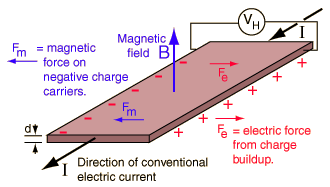
\includegraphics[scale=.8]{hall.png}
      \caption{Image from {\url http://hyperphysics.phy-astr.gsu.edu/hbase/magnetic/imgmag/hall.gif}}
      \label{fig:hall_effect}
\end{figure}

\end{document}